\label{subsec:sw2}
The smartwatch that was chosen to do the project with is the Sony 
SmartWatch 2. It is a cheap watch and it is programmable. The SDK has recently been updated and is easy to use. We have used the SDK to quickly make an application. There are many examples which are easily installed. The installation give can be found at this website \cite{sw2_install}. These examples were used to generate traffic for the Ubertooth to detect. This sped up the process of finding targeting and decoding the packets. 
\begin{figure}[!h]
  \begin{center}
	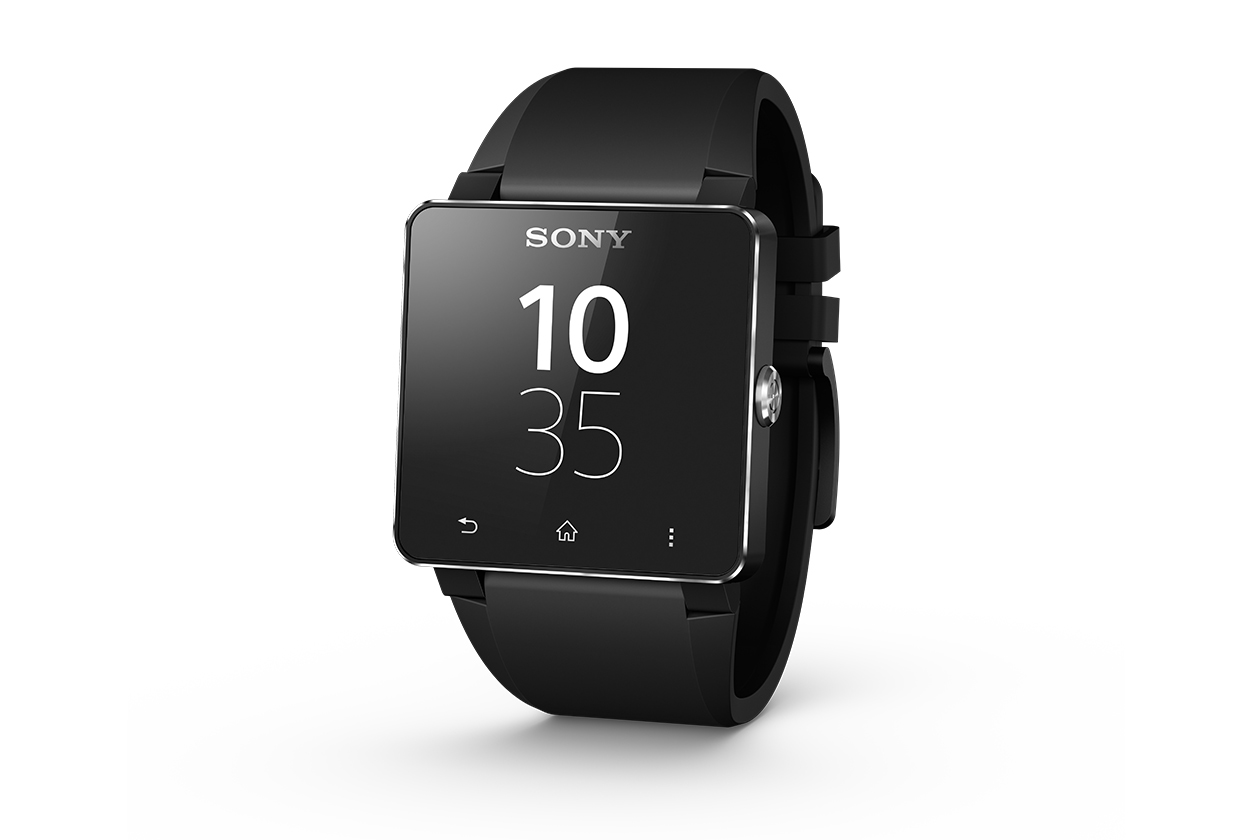
\includegraphics[width=200px]{images/sw2.jpg}
	\label{fig:sw2}
	\caption{The smartwatch we are investigating}
  \end{center}
\end{figure}
\\

The smartwatch uses Bluetooth 3.0. The SDK has recently been updated so it still in active development and is easy to use. We have used the SDK to quickly make an application. There are many example applications which are easily installed. These examples were used to generate traffic for the Ubertooth to detect. This sped up the process of finding targeting and decoding the packets. \pend
All the Sony devices use an application called Smart Connect. This application keeps track of all the devices that want to make contact with the phone. It also keeps track of the applications that are installed on the watch. Whenever the pairing is stopped between the phone and the watch all the previous installed applications are removed from the watch until they are paired again.
\subsubsection{Smartwatch applications}
\label{subsubsec:sw_app}
%needs revision
The life cycle of a smartwatch app is about the same as an application on a phone or tablet. This can be seen in figure \ref{fig:sw2_lifecycle}. Like stated before the smartwatch apps only work when they are paired with the master device(the device which has the Smart Connect installed). When making an app you need to do a few things. First you have to register the app. This registration is needed for Smart Connect to find the app. \pend
Then you have to update your AndroidManifest.xml where you will tell which activity is your main activity and some control features. After this you can start working on your by including the mandatory classes to make the application compatible with SW2. \pend  
Sony has made a level of abstraction that makes it easy to send messages using intents. As stated before the pairing process is handled by the Smart Connect. 
\begin{figure}
\begin{center}
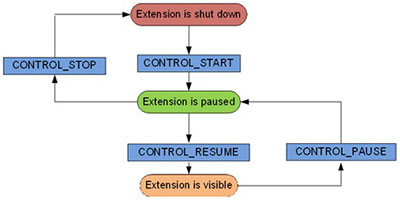
\includegraphics[scale=0.5]{images/applifecycle.jpg}
\end{center}
  \caption{Life cycle of a Sony smartwatch app}
  \label{fig:sw2_lifecycle}
  \captionsetup{font={footnotesize,bf,it}}
  \caption*{\url{https://developer.sony.com/develop/wearables/smartwatch-2-apis/guides/build-your-app/}}
\end{figure}